%======================================================================
% GMI-15 Integralni vety.pdf
%======================================================================
% symbol hustoty (v originále pětiúhelník otevřený doleva)
\providecommand{\gmIpatnactHust}{\mathord{\tikz[baseline=0pt,x=0.85ex,y=0.85ex,line width=0.45pt]{\draw (0,0.6)--(0.45,1.15)--(1.5,1.15)--(1.5,0.05)--(0.45,0.05)--cycle;}}}

\section{Integrální věty}
\strana{GMI-15-1}

\begin{itemize}[nosep]
  \item Podvariety a přizpůsobené souřadnice
  \item Integrování AS forem na podvarietě
  \item Integrování AS tenzorových hustot na podvarietě
  \item Integrální věty
  \item Ortogonální rozštěpení na nadploše
\end{itemize}

%----------------------------------------------------------------------
\strana{GMI-15-2}
\subsection{Podvariety a přizpůsobené souřadnice}

\kw{podvarieta} \quad $N\subset M$ \\
\quad $\dim M = m$, \quad $\dim N = n$, \quad \kw{kodimenze} \ $\hat n = m - n$

tečné vektory \\
\quad $\mathbf{T}_xN\subset\mathbf{T}_xM$ \quad lze vnořit jako podprostor $\mathbf{T}_xM$ \\
\quad \pozor{normálové vektory nelze kanonicky identifikovat jako podprostor $\mathbf{T}_xM$}

normálové formy \\
\quad $\mathbf{N}^*_xN\subset\mathbf{T}^*_xM$ \quad lze vnořit jako podprostor $\mathbf{T}^*_xM$ \\
\quad \pozor{tečné formy nelze kanonicky identifikovat jako podprostor $\mathbf{T}^*_xM$}

\begin{minipage}{0.58\textwidth}
\kw{přizpůsobené souřadnice} \quad (konvence norm--teč)

\begin{tabular}{@{}lll}
$x^a$ & souř.\ v $M$ & $a,b,\ldots = 1,\ldots,m$ \\
$x^u = \text{konst.}$ & & $u,v,\ldots = 1,\ldots,\hat n$ \\
\multicolumn{2}{@{}l}{\quad vazby určující $N$} & \\
$x^i$ & souř.\ v $N$ & $i,j,\ldots = \hat n+1,\ldots,\hat n+n$
\end{tabular}
\end{minipage}
\begin{minipage}{0.4\textwidth}
\begin{tikzpicture}[scale=0.9]
  % krabice M
  \draw (0,0) -- (3,0) -- (3,2) -- (0,2) -- cycle;
  \draw (0,2) -- (1,2.7) -- (4,2.7) -- (3,2);
  \draw (3,0) -- (4,0.7) -- (4,2.7);
  \draw[gray!60] (0,0) -- (1,0.7) -- (4,0.7);
  \draw[gray!60] (1,0.7) -- (1,2.7);
  % podvarieta N (vodorovný řez)
  \draw[thick] (0,1) -- (3,1) -- (4,1.7);
  \draw[thick,gray] (0,1) -- (1,1.7) -- (4,1.7);
  \node[below] at (1.7,0.95) {$N$};
  \node[below right] at (3.4,0) {$M$};
  % souřadnice
  \draw[-{Stealth}] (2.2,1.3) -- (2.8,1.5) node[right] {\small $x^i$};
  \draw[-{Stealth}] (2.2,1.3) -- (2.5,1.05);
  \draw[-{Stealth}] (4.2,1.7) -- (4.2,2.4) node[right] {\small $x^u$};
\end{tikzpicture}
\end{minipage}

\begin{vysvetleni}[Podvarieta, tečné a normálové směry]
$N$ je $n$-rozměrná plocha v $m$-rozměrné $M$; kodimenze $\hat n$ je počet vazeb, které ji vymezují. Tečný vektor k $N$ je zároveň vektorem v $M$ (vnoření $\mathbf T_xN\hookrightarrow\mathbf T_xM$). Normálové formy jsou kovektory, které anulují všechny tečné vektory k $N$ (např.\ gradienty vazeb $\dd x^u$) -- ty tvoří podprostor $\mathbf N^*_xN\subset\mathbf T^*_xM$. Naopak „normálový vektor“ či „tečnou formu“ bez dodatečné struktury (metriky) jednoznačně vybrat nelze: normálové vektory jsou jen třídy $\mathbf T_xM/\mathbf T_xN$ a tečné formy jen restrikce kovektorů z $M$. Metrika toto rozštěpení doplní -- viz poslední oddíl (GMI-15-7).

Přizpůsobené souřadnice: prvních $\hat n$ souřadnic ($x^u$) je konstantních na $N$, zbylých $n$ ($x^i$) parametrizuje $N$ (konvence „nejdřív normálové, pak tečné“). Krtouš (odd.~5.8, D3.15) používá jiné písmena: $d=\dim M$, $n$ = kodimenze, $\dim N=d-n$, se stejným pořadím (vazby $x^1,\ldots,x^n$ první).
\end{vysvetleni}

\kw{tenzor orientace} na $M$ a $N$
\begin{align*}
  \tilde\varepsilon_M &= (\dd^m x)^{-1}\,\dd x^1\wedge\ldots\wedge\dd x^m &
  \tilde\varepsilon_M^{-1} &= \dd^m x\,\pdv{x^1}\wedge\ldots\wedge\pdv{x^m} \\
  \tilde\varepsilon_N &= (\dd^n x)^{-1}\,\dd x^{\hat n+1}\wedge\ldots\wedge\dd x^{\hat n+n} &
  \tilde\varepsilon_N^{-1} &= \dd^n x\,\pdv{x^{\hat n+1}}\wedge\ldots\wedge\pdv{x^{\hat n+n}}
\end{align*}

\begin{vysvetleni}[Tenzor orientace]
$\tilde\varepsilon_M$ je maximální AS forma s „hustotní vahou $-1$“ (prvek $\mathbf H^{-1}M\otimes\Lambda^mM$): faktor $(\dd^mx)^{-1}$ ruší Jacobián, který vznikne při přechodu k jiným souřadnicím ve formě $\dd x^1\wedge\ldots\wedge\dd x^m$. Výsledek tak nezávisí na souřadnicích, pouze na orientaci -- nese tedy jen informaci o orientaci, nikoli o „objemu“. $\tilde\varepsilon_M^{-1}\in\mathbf H M\otimes\mathbf T^{[m]}M$ je inverzní objekt ($\tilde\varepsilon_M\bullet\tilde\varepsilon_M^{-1}=1$). Jejich pomocí se zavádí hustotní duál $*$ mezi AS formami a AS tenzorovými hustotami (Krtouš, odd.~5.5--5.6). Na $N$ se totéž definuje se souřadnicemi $x^i$; souřadnice musí být kladně orientované vůči oběma orientacím.
\end{vysvetleni}

tečné vektory \\
\quad lin.\ obal \quad $\pdv{x^{\hat n+1}},\ldots,\pdv{x^{\hat n+n}}$

normálové formy \\
\quad lin.\ obal \quad $\dd x^1,\ldots,\dd x^{\hat n}$

\begin{definice}[Restrikce AS formy na podvarietu]
$\omega\in\Lambda^pM \;\to\; \omega|_N\in\Lambda^pN$ \quad dané akcí $\omega$ na tečných vektorech
\begin{align*}
  \omega &= \sum_{k_1<\ldots<k_p}\omega_{k_1\ldots k_p}\,\dd x^{k_1}\wedge\ldots\wedge\dd x^{k_p} &&\in\Lambda^pM \\
  \downarrow\ \ & \\
  \omega|_N &= \sum_{\hat n<k_1<\ldots<k_p}\omega_{k_1\ldots k_p}\,\dd x^{k_1}\wedge\ldots\wedge\dd x^{k_p} &&\in\Lambda^pN
\end{align*}
\end{definice}

\begin{vysvetleni}[Restrikce = pullback]
Restrikce $\omega|_N$ je zpětný přenos (pullback) formy vnořením $N\hookrightarrow M$: forma se smí „krmit“ jen tečnými vektory k $N$. V přizpůsobených souřadnicích na $N$ platí $\dd x^u|_N=0$ ($x^u$ jsou na $N$ konstantní), takže ze součtu přežijí jen členy, kde jsou všechny indexy tečné ($k_1>\hat n$). Tečné formy tak nejsou podprostorem $\mathbf T^*M$, ale kvocientem -- formy lišící se jen o normálové části mají stejnou restrikci. Viz Krtouš, D3.16 a vztah (5.20).
\end{vysvetleni}

%----------------------------------------------------------------------
\strana{GMI-15-3}
\subsection{Integrování AS forem na podvarietě}

AS $n$-forma určuje integrovatelnou hustotu na podvarietě $N$

\begin{tabular}{@{}ll}
$\alpha\in\Lambda^nM$ & obsahuje složky ve všech směrech v $M$ \\
$\alpha|_N\in\Lambda^nN$ & obsahuje pouze složky tečné k $N$ \\
$\gmIpatnactHust = \iota_+\alpha|_N\in\mathbf{H}N$ & odpovídající hustota, kterou lze integrovat na $N$
\end{tabular}

\quad $\alpha\to\alpha|_N\to\gmIpatnactHust = \tilde\varepsilon_N^{-1}\bullet\alpha|_N$ \quad
lze zakódovat do \\
\hspace*{5.6cm} \kw{tečného objemového (plošného) elementu} $\dd\Sigma_N$
\[
  \vzorec{\gmIpatnactHust = \alpha\bullet\dd\Sigma_N}
\]
\quad $\dd\Sigma_N$ je ekvivalent $\tilde\varepsilon_N^{-1}$ s vektorovými indexy chápanými v $\mathbf{T}M$
\[
  \dd\Sigma_N\in\mathbf{H}_xN\otimes\mathbf{T}^{[n]}_xM
\]
\[
  \dd\Sigma_N = \dd^n x\,\underbrace{\pdv{x^{\hat n+1}}\wedge\ldots\wedge\pdv{x^{\hat n+n}}}_{\text{chápáno jako vektory v }\mathbf{T}_xM}
  \qquad\leftarrow\qquad
  \tilde\varepsilon_N^{-1} = \dd^n x\,\underbrace{\pdv{x^{\hat n+1}}\wedge\ldots\wedge\pdv{x^{\hat n+n}}}_{\text{chápáno jako vektory v }\mathbf{T}_xN}
\]
\[
  \gmIpatnactHust = \alpha_{\hat n+1\ldots\hat n+n}\,\dd^n x
\]

\begin{vysvetleni}[Tečný objemový element $\dd\Sigma_N$]
Symbol $\gmIpatnactHust$ (pětiúhelník) značí v poznámkách obecně \emph{hustotu} / tenzorovou hustotu; zde konkrétně hustotu na $N$. Izomorfismus $\iota_+:\Lambda^nN\to\mathbf HN$ nahradí $\dd x^{\hat n+1}\wedge\ldots\wedge\dd x^{\hat n+n}$ hustotou $\dd^nx$ (pro kladně orientované souřadnice), tj.\ $\iota_+\beta=\tilde\varepsilon_N^{-1}\bullet\beta$; $\bullet$ je úplné zúžení přes všechny AS indexy (s normalizací $1/n!$, Krtouš odd.~5.6).

$\dd\Sigma_N$ spojuje oba kroky -- restrikci i $\iota_+$ -- do jednoho objektu: je to $\tilde\varepsilon_N^{-1}$, jehož vektorová část je vnořena do $\mathbf T M$, takže jej lze zúžit přímo s formou $\alpha$ na $M$; zúžení s tečnými vektory automaticky vybere jen tečnou složku $\alpha_{\hat n+1\ldots\hat n+n}$. Hustota $\dd^nx$ zůstává hustotou na $N$. Viz Krtouš, D5.22--D5.23 a (5.24)--(5.26). Pro křivku je to známé $\int\vec A\cdot\dd\vec l$: výsledek nezávisí na parametrizaci, protože $\pdv{\tau}$ a $\dd\tau$ se při změně $\tau$ transformují inverzně.
\end{vysvetleni}

\begin{minipage}{0.6\textwidth}
integrování tečné složky AS formy
\[
  \vzorec{\int_{V\subset N}\alpha|_N = \int_{V\subset N}\alpha\bullet\dd\Sigma_N}
\]
\end{minipage}
\begin{minipage}{0.38\textwidth}
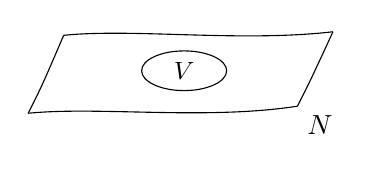
\begin{tikzpicture}[scale=0.9]
  \draw (0,0) .. controls (1,0.1) and (2.5,-0.1) .. (3.8,0.1);
  \draw (0.5,1.1) .. controls (1.5,1.2) and (3,1.0) .. (4.3,1.15);
  \draw (0,0) .. controls (0.2,0.4) .. (0.5,1.1);
  \draw (3.8,0.1) .. controls (4.0,0.5) .. (4.3,1.15);
  \draw (2.2,0.6) ellipse (0.6 and 0.28);
  \node at (2.2,0.6) {\small $V$};
  \node[below right] at (3.8,0.1) {$N$};
\end{tikzpicture}
\end{minipage}

\begin{priklad}[Př.]
$\dd\Sigma_N$ je zobecnění $\dd\vec l = \vec t\,\dd l$ pro křivky

$\dim N = n = 1$, \quad $\tau$ souř.\ na $N$, \quad
$\tilde\varepsilon^{-1} = \dd\tau\,\pdv{\tau}$ \quad (hustota na $N$)
\[
  \dd\Sigma_N = \underbrace{\pdv{\tau}}_{\text{tečný vekt.\ k }N}\ \underbrace{\dd\tau}_{\text{hustota na }N}
  \qquad\leftarrow\ \text{nezávisí na parametrizaci }\tau
\]
\[
  \int_{I\subset N}\alpha\bullet\dd\Sigma_N = \int_{I\subset N}\alpha_\tau\,\dd\tau
\]
\end{priklad}

%----------------------------------------------------------------------
\strana{GMI-15-4}
\subsection{Integrování AS tenzorových hustot na podvarietě}

AS $\hat n$-tenzorová hustota určuje integrovatelnou hustotu na $N$

\begin{tabular}{@{}ll}
$\gmIpatnactHust\in\Lambda^{*\hat n}M$ & obsahuje složky ve všech směrech v $M$ \\
$\gmIpatnactHust|_N\in\mathbf{H}N$ & obsahuje pouze normálové složky k $N$ \\
 & jedná se o hustotu, kterou lze integrovat na $N$
\end{tabular}

definujeme pomocí duality k AS formám
\[
  \gmIpatnactHust|_N = \gmIpatnactHust\bullet\dd\tilde S_N = \alpha\bullet\dd\Sigma_N
  \qquad\text{kde}\quad \alpha = {*}\gmIpatnactHust = \gmIpatnactHust\bullet\tilde\varepsilon_M
\]
\[
  \dd\tilde S_N\in
  \underbrace{\mathbf{H}_xN}_{\text{hustota na }N}\otimes
  \underbrace{\mathbf{H}^{-1}_xM}_{\text{ruší hustotní charakter na }M}\otimes
  \underbrace{\mathbf{N}^*N}_{\text{vybírá normálové složky}}
\]
\[
  \vzorec{\dd\tilde S_N = \tilde\varepsilon_M\bullet\dd\Sigma_N}
  = \dd^n x\,(\dd^m x)^{-1}\,\dd x^1\wedge\ldots\wedge\dd x^{\hat n}
\]
\[
  \gmIpatnactHust|_N = \gmIpatnactHust_x^{1\ldots\hat n}\,\dd^n x
\]

\begin{vysvetleni}[Normálový objemový element $\dd\tilde S_N$]
$\Lambda^{*\hat n}M$ zde značí AS tenzorové hustoty řádu $\hat n$ (prvky $\mathbf HM\otimes\mathbf T^{[\hat n]}M$, např.\ pro $\hat n=1$ „vektorová hustota“ jako $\vec j\,\dd^mx$). Takovou hustotu nelze restringovat na $N$ jako formu, ale lze ji převést hustotním duálem $*$ na $(m-\hat n)=n$-formu $\alpha$ a tu integrovat pomocí $\dd\Sigma_N$. $\dd\tilde S_N=\tilde\varepsilon_M\bullet\dd\Sigma_N$ tento převod „předpočítá“: má $\hat n$ normálových kovektorových indexů (vybírá složky $\gmIpatnactHust^{1\ldots\hat n}$ ve směrech \emph{ven} z $N$), faktor $(\dd^mx)^{-1}$ odstraní hustotní váhu na $M$ a $\dd^nx$ dodá hustotu na $N$. Dolní index $x$ u $\gmIpatnactHust_x^{1\ldots\hat n}$ znamená „složka vůči souřadnicím $x$“ (tj.\ koeficient u $\pdv{x^1}\wedge\ldots\wedge\pdv{x^{\hat n}}\,\dd^mx$). Viz Krtouš, D5.24--D5.25, (5.27)--(5.29). Pro nadplochu v $\mathbb E^3$ dostaneme klasický tok $\int\vec j\cdot\dd\vec S$.
\end{vysvetleni}

\begin{minipage}{0.6\textwidth}
integrování normálové složky AS tenzorové hustoty
\[
  \vzorec{\int_{V\subset N}\gmIpatnactHust|_N = \int_{V\subset N}\gmIpatnactHust\bullet\dd\tilde S_N}
\]
\end{minipage}
\begin{minipage}{0.38\textwidth}
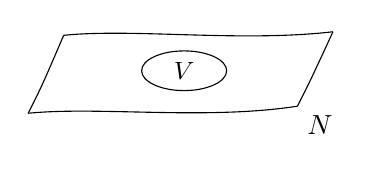
\begin{tikzpicture}[scale=0.9]
  \draw (0,0) .. controls (1,0.1) and (2.5,-0.1) .. (3.8,0.1);
  \draw (0.5,1.1) .. controls (1.5,1.2) and (3,1.0) .. (4.3,1.15);
  \draw (0,0) .. controls (0.2,0.4) .. (0.5,1.1);
  \draw (3.8,0.1) .. controls (4.0,0.5) .. (4.3,1.15);
  \draw (2.2,0.6) ellipse (0.6 and 0.28);
  \node at (2.2,0.6) {\small $V$};
  \node[below right] at (3.8,0.1) {$N$};
\end{tikzpicture}
\end{minipage}

\begin{priklad}[Př.]
$\dd\tilde S_N$ je zobecnění $\dd\vec S = \vec n\,\dd S$ pro (nad)plochy

$\dim N = n = m-1$, \quad $\hat n = 1$
\[
  \dd\tilde S_N = \underbrace{\frac{\dd^{m-1}x}{\dd^m x}}_{\substack{\text{převádí hustotu na }M\\\text{na hustotu na }N}}\
  \underbrace{\dd x^1}_{\text{normálová 1-forma}}
  \qquad\leftarrow\ \text{nezávisí na volbě vazby } x^1 = \text{konst}
\]
\[
  \int_{V\subset N}\gmIpatnactHust\bullet\dd\tilde S_N = \int_{V\subset N}\gmIpatnactHust_x^1\,\dd^{m-1}x
\]
\end{priklad}

\textbf{Př:} Pro $M = N$, tj.\ $m = n$, $\hat n = 0$, je $\dd\tilde S_M$ triviální: \ $\dd\tilde S_M = 1$

\textbf{vztah tečných a normálových složek AS forem a tenz.\ hustot}
\[
  \gmIpatnactHust = {*}\alpha \quad\Rightarrow\quad
  \gmIpatnactHust_x^{\hat K} = \tilde\varepsilon_{Mx}^{-1\,\hat KK}\alpha_K
  \qquad\text{nesčítá se (1 sčítanec), } \hat K, K \text{ doplňkové}
\]
\[
  \Rightarrow\quad
  \underbrace{\gmIpatnactHust_x^{1\ldots\hat n}}_{\text{normálová složka }\gmIpatnactHust} =
  \underbrace{\alpha_{\hat n+1\ldots\hat n+n}}_{\text{tečná složka }\alpha}
  \qquad\text{jelikož}\quad \tilde\varepsilon_{Mx}^{-1\,1\ldots\hat n\ldots m} = 1
\]

\begin{vysvetleni}[Proč normálová složka = tečná složka]
$K$, $\hat K$ jsou multiindexy (uspořádané množiny indexů) navzájem doplňkové v $\{1,\ldots,m\}$. Hustotní duál přiřadí složce formy $\alpha_K$ složku hustoty s „chybějícími“ indexy $\hat K$, se znaménkem permutace $(\hat K,K)$. Díky konvenci „nejdřív normálové, pak tečné souřadnice“ je pro $\hat K=(1,\ldots,\hat n)$, $K=(\hat n+1,\ldots,m)$ permutace identická a znaménko $+1$. Proto $\gmIpatnactHust\bullet\dd\tilde S_N=({*}\gmIpatnactHust)\bullet\dd\Sigma_N$ -- integrál toku hustoty přes $N$ je totéž co integrál duální formy přes $N$ (Krtouš, lemma V5.9\,(i)).
\end{vysvetleni}

%----------------------------------------------------------------------
\strana{GMI-15-5}
\subsection{Integrální věty}

\begin{minipage}{0.68\textwidth}
\begin{veta}[Stokesova věta pro AS formy]
\[
  \vzorec{\int_\Omega\dd\omega = \int_{\partial\Omega}\omega|_{\partial\Omega}}
  \qquad \omega\in\Omega^{m-1}M
\]
\end{veta}
základní forma integrální věty \\
komentář k důkazu -- viz \% \pozn{odkaz nejasný}
\end{minipage}
\begin{minipage}{0.3\textwidth}
\centering
\begin{tikzpicture}[scale=0.9]
  \draw (0,0) ellipse (0.95 and 0.8);
  \draw (-0.65,-0.1) .. controls (-0.3,-0.35) and (0.3,-0.35) .. (0.65,-0.1);
  \node at (0,0.15) {$\Omega$};
  \draw[dashed,gray] (-0.45,0.25) .. controls (-0.2,0.32) and (0.2,0.32) .. (0.45,0.25);
  \draw[-{Stealth}] (1.6,0.75) .. controls (1.1,0.85) and (0.7,0.65) .. (0.45,0.48);
  \node[right] at (1.6,0.75) {$\partial\Omega$};
\end{tikzpicture}
\end{minipage}

\begin{vysvetleni}[Stokesova věta]
$\Omega\subset M$ je $m$-rozměrná oblast s hranicí $\partial\Omega$ (dimenze $m-1$), $\omega$ je $(m-1)$-forma; vpravo stojí její restrikce (pullback) na hranici. Hranice musí být orientována indukovaně: kladně orientovaná báze na $\partial\Omega$ doplněná \emph{napřed} vnější normálou dává kladnou orientaci $M$. Věta zobecňuje Newtonův (Leibnizův) vzorec $\int_a^bf'=f(b)-f(a)$ ($m=1$, $\omega=f$, hranice dvoubodová se znaménky $\pm$); všechny klasické integrální věty (Green, Stokes, Gauss--Ostrogradskij) jsou její speciální případy -- viz Krtouš, V10.14 a P10.1. Symbol „\%“ v odkazu nejspíš míní pozdější stranu s nástinem důkazu (GMI-15-6).
\end{vysvetleni}

\begin{minipage}{0.6\textwidth}
\begin{veta}[Stokesova věta pro AS formy na podvarietě]
\[
  \vzorec{\int_{V\subset N}\dd\alpha|_N = \int_{\partial V}\alpha|_{\partial V}}
  \qquad \alpha\in\Omega^{\oprava{n-1}{m-1}}M
\]
\end{veta}
\end{minipage}
\begin{minipage}{0.38\textwidth}
\centering
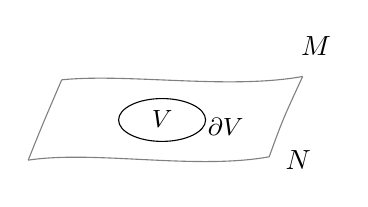
\begin{tikzpicture}[scale=0.85]
  \draw[gray] (0,0) .. controls (1,0.15) and (2.5,-0.15) .. (3.6,0.05);
  \draw[gray] (0.5,1.2) .. controls (1.5,1.3) and (3,1.05) .. (4.1,1.25);
  \draw[gray] (0,0) .. controls (0.2,0.5) .. (0.5,1.2);
  \draw[gray] (3.6,0.05) .. controls (3.8,0.6) .. (4.1,1.25);
  \draw (2,0.6) ellipse (0.65 and 0.32);
  \node at (2,0.62) {\small $V$};
  \node at (2.95,0.5) {\small $\partial V$};
  \node[right] at (3.7,0.0) {$N$};
  \node at (4.3,1.7) {$M$};
\end{tikzpicture}
\end{minipage}

vnější derivace komutuje s restrikcí \\
postupné restrikce na $N$ a $\partial V$ je ekvivalentní restrikci přímo na $\partial V$

\begin{vysvetleni}[Stokes na podvarietě]
Oprava stupně: integrand $\dd\alpha|_N$ se integruje přes $n$-rozměrnou $V$, musí to tedy být $n$-forma, a $\alpha$ je proto $(n-1)$-forma na $M$ (u Krtouše V10.14: $\omega\in\Lambda^{d-p}M$, $\dim N=d-p+1$). Pro $N=M$ to splývá s předchozí větou.

Věta plyne z té předchozí aplikované na formu $\alpha|_N$ na varietě $N$: restrikce je pullback a pullback komutuje s vnější derivací, $(\dd\alpha)|_N=\dd(\alpha|_N)$, a restrikce na $N$ a pak na $\partial V$ je pullback složeným vnořením $\partial V\hookrightarrow N\hookrightarrow M$, tedy $(\alpha|_N)|_{\partial V}=\alpha|_{\partial V}$.
\end{vysvetleni}

\begin{veta}[Stokesova věta s rotací]
\[
  \vzorec{\int_{V\subset N}\widetilde{\operatorname{rot}}\,\alpha\bullet\dd\tilde S_N = \int_{\partial V}\alpha\bullet\dd\Sigma_{\partial V}}
\]
\end{veta}
\begin{align*}
  \text{levé str.:}\quad &\int_{V\subset N}\widetilde{\operatorname{rot}}\,\alpha\bullet\dd\tilde S_N
   = \int_{V\subset N}({*}\dd\alpha)\bullet\dd\tilde S_N
   = \int_{V\subset N}(\dd\alpha)\bullet\dd\Sigma_N
   = \int_{V\subset N}\dd\alpha|_N \\
  \text{pravé str.:}\quad &\int_{\partial V}\alpha\bullet\dd\Sigma_{\partial V} = \int_{\partial V}\alpha|_{\partial V}
\end{align*}

\begin{vysvetleni}[Rotace a důkaz]
$\widetilde{\operatorname{rot}}\,\alpha={*}\dd\alpha$ je hustotní duál vnější derivace -- AS tenzorová hustota řádu $m-n=\hat n$ (vlnka zdůrazňuje hustotní charakter); viz Krtouš D10.1. Důkaz je jen přepis Stokesovy věty pro formy: na levé straně se použije vztah $({*}\beta)\bullet\dd\tilde S_N=\beta\bullet\dd\Sigma_N$ z GMI-15-4 (Krtouš, V5.9\,(i)), na pravé definice $\dd\Sigma_{\partial V}$. Pro $m=3$, $n=2$, $\alpha=\vec A\cdot\dd\vec x$ s euklidovskou metrikou dostaneme klasické $\int_S(\nabla\times\vec A)\cdot\dd\vec S=\oint_{\partial S}\vec A\cdot\dd\vec l$ (Krtouš (10.6a)).
\end{vysvetleni}

\begin{veta}[Gaussova věta]
\[
  \vzorec{\int_{V\subset N}(\operatorname{div}\gmIpatnactHust)\bullet\dd\tilde S_N = \int_{\partial V}\gmIpatnactHust\bullet\dd\tilde S_{\partial V}}
\]
\end{veta}
\begin{align*}
  \text{levé str.:}\quad &\int_{V\subset N}(\operatorname{div}\gmIpatnactHust)\bullet\dd\tilde S_N
   = \int_{V\subset N}({*}\dd\alpha)\bullet\dd\tilde S_N
   = \int_{V\subset N}(\dd\alpha)\bullet\dd\Sigma_N
   = \int\dd\alpha|_N
   && \text{pro } \alpha = {*}\gmIpatnactHust \\
  \text{pravé str.:}\quad &\int_{\partial V}\gmIpatnactHust\bullet\dd\tilde S_{\partial V}
   = \int_{\partial V}({*}\alpha)\bullet\dd\tilde S_{\partial V}
   = \int_{\partial V}\alpha\bullet\dd\Sigma_{\partial V}
   = \int_{\partial V}\alpha|_{\partial V}
\end{align*}

\begin{vysvetleni}[Divergence a Gaussova věta]
Divergence AS tenzorové hustoty je $\operatorname{div}\gmIpatnactHust={*}\dd{*}\gmIpatnactHust$ (Krtouš D10.1) -- snižuje řád o 1 a nepotřebuje metriku ani konexi. Aby šlo levou stranu integrovat přes $N$ (kodimenze $\hat n$), musí být $\operatorname{div}\gmIpatnactHust$ řádu $\hat n$, tedy $\gmIpatnactHust$ řádu $\hat n+1$ a na hranici $\partial V$ (kodimenze $\hat n+1$) se integruje přímo $\gmIpatnactHust$. Pro $\alpha={*}\gmIpatnactHust$ je $\operatorname{div}\gmIpatnactHust={*}\dd\alpha$ a obě strany se převedou na Stokesovu větu pro $\alpha$ (využívá se ${*}{*}=1$ pro hustotní duál). Krtouš, V10.16.
\end{vysvetleni}

\begin{veta}[Gaussova věta v maximální dim.]
\[
  \vzorec{\int_\Omega\operatorname{div}\gmIpatnactHust = \int_{\partial\Omega}\gmIpatnactHust\bullet\dd\tilde S_{\partial\Omega}}
\]
pro $M = N$: \quad $\dd\tilde S_M = 1$, \quad $\gmIpatnactHust\in\Lambda^{*1}M$, \quad $\operatorname{div}\gmIpatnactHust\in\mathbf{H}M$
\end{veta}

\begin{vysvetleni}[Klasická Gaussova věta]
Pro $N=M$ je $\gmIpatnactHust$ vektorová hustota, v souřadnicích $\gmIpatnactHust=\gmIpatnactHust^a\pdv{x^a}\,\dd^mx$, a $\operatorname{div}\gmIpatnactHust=\partial_a\gmIpatnactHust^a\,\dd^mx$ -- obyčejné parciální derivace stačí, protože jde o hustotu (bez metriky). Vpravo je tok přes hranici s $\dd\tilde S_{\partial\Omega}$ jako „$\vec n\,\dd S$“ bez metriky. S metrikou viz konec této kapitoly (GMI-15-7), Krtouš (10.7).
\end{vysvetleni}

%----------------------------------------------------------------------
\strana{GMI-15-6}
\subsubsection*{Stokesova věta -- nástin důkazu}

\begin{minipage}{0.5\textwidth}
\[
  \int_{V\subset N}\dd\alpha|_N = \int_{\partial V}\alpha|_{\partial V}
\]

\kw{nástin linie důkazu}
\begin{itemize}[nosep]
  \item[--] rozřezat $V$ na oblasti v souř.\ mapách
  \item[--] hranice $\partial V$ pouze ve směru $x^{\hat n+1}$
  \item[--] $\alpha$ vymizí na $\partial U$
\end{itemize}
\end{minipage}
\begin{minipage}{0.48\textwidth}
\centering
\begin{tikzpicture}[scale=0.85]
  % podvarieta N
  \draw (0,0.6) -- (3.6,1.5) -- (5.4,0.2) -- (1.8,-0.7) -- cycle;
  \node at (5.2,-0.2) {$N$};
  \node at (5.4,2.9) {\Large $M$};
  % oblast V
  \draw (2.0,0.35) ellipse (0.75 and 0.55);
  \node at (1.75,0.3) {$V$};
  \node at (1.7,-0.45) {\small $\partial V$};
  % mapa U (svislá elipsa)
  \draw[thick] (3.05,1.0) ellipse (0.65 and 1.95);
  \draw[dashed,gray] (2.4,0.55) .. controls (2.7,0.1) and (3.4,0.1) .. (3.7,0.55);
  \node at (3.5,-1.1) {$U$};
  % průnik U s N
  \draw (2.95,0.45) ellipse (0.55 and 0.4);
  % osy
  \draw[-{Stealth}] (3.0,2.0) -- (3.0,2.8);
  \node at (2.2,3.2) {\small $x^1\ldots x^{\hat n}$};
  \draw[gray] (2.5,3.05) .. controls (2.7,2.9) .. (2.95,2.7);
  \draw[-{Stealth}] (2.85,0.55) -- (3.6,0.75) node[right] {\small $x^{\hat n+1}$};
  \draw[-{Stealth}] (2.85,0.55) -- (3.0,0.2);
  \node at (1.4,2.5) {\small $x^{\hat n+2}\ldots x^{\hat n+n}$};
  \draw[gray] (1.8,2.3) .. controls (2.3,1.6) and (2.6,1.0) .. (2.85,0.6);
\end{tikzpicture}
\end{minipage}

\begin{align*}
  \int_{V\subset N}\dd\alpha|_N
  &= \int_{V\subset N}(\dd\alpha)_{\hat n+1\ldots\hat n+n}\,\dd^n x = \\
  &= \int_{V\subset N}\sum_{k=1}^{n}(-1)^{k+1}\,
     \alpha_{\underbrace{\scriptstyle\hat n+1\ldots\hat n+n}_{\text{mimo }\hat n+k},\,\hat n+k}\,
     \dd x^{\hat n+k}\,\dd^{n-1}x
\end{align*}
\quad Newtonův vzorec $\to$ okrajové členy \\
\quad vymizí pro $k = 2\ldots n$ \\
\quad příspěvek pouze na hranici $\partial V$
\begin{align*}
  &= \int_{V\subset N}\alpha_{\hat n+2\ldots\hat n+n,\,\hat n+1}\,\dd x^{\hat n+1}\,\dd^{n-1}x \\
  &= \int_{\partial V}\alpha_{\hat n+2\ldots\hat n+n}\,\dd^{n-1}x \\
  &= \int_{\partial V}\alpha|_{\partial V}
\end{align*}

\begin{vysvetleni}[Jak číst nástin důkazu]
Pomocí rozkladu jednotky se $\alpha$ rozloží na součet forem, z nichž každá má nosič v jedné souřadnicové mapě $U$ (proto „$\alpha$ vymizí na $\partial U$“). V $U$ se zvolí přizpůsobené souřadnice tak, aby $\partial V$ byla dána podmínkou $x^{\hat n+1}=\text{konst}$ a $x^{\hat n+1}$ rostla směrem ven z $V$. Čárka v indexu značí parciální derivaci: $\alpha_{\ldots,\hat n+k}=\partial_{\hat n+k}\alpha_{\ldots}$; součet se znaménky $(-1)^{k+1}$ je souřadnicový tvar $(\dd\alpha)_{\hat n+1\ldots\hat n+n}$. Integrál přes $x^{\hat n+k}$ se spočte Newtonovým vzorcem; pro $k\ge2$ dá hodnoty na $\partial U$, kde $\alpha=0$, jen pro $k=1$ zbude hodnota na $\partial V$. Zbylý integrál přes $x^{\hat n+2},\ldots,x^{\hat n+n}$ je $\int_{\partial V}\alpha|_{\partial V}$ s orientací „vnější normála první“. Zde $\dd^{n-1}x=\dd x^{\hat n+2}\cdots\dd x^{\hat n+n}$.
\end{vysvetleni}

%----------------------------------------------------------------------
\strana{GMI-15-7}
\subsection{Ortogonální rozštěpení na nadploše}

$g$ -- metrika na $M$ \\
\quad definuje ortogonální rozštěpení na norm.\ a tečné směry \\
\quad\quad $n$ je normálový vekt.\ $\Leftrightarrow$ \ $n\cdot g\cdot t = 0$ \ $\forall t$ tečný \\
\quad\quad $\sigma$ je tečný kovektor $\Leftrightarrow$ \ $\sigma\cdot g^{-1}\cdot\nu = 0$ \ $\forall\nu$ normál.\
$\Leftrightarrow$ \ $\sigma\cdot n = 0$ \ $\forall n$ norm. \\
\quad umožňuje normalizaci normál

\kw{nadplochy}: \quad $\dim N = n = m-1$, \quad $\hat n = 1$ \hfill $M, N$ orientovatelné \\
\quad dim normál $= 1$, \quad dim tečných $= m-1$

\textbf{rozštěpení metriky}

\begin{tabular}{@{}l@{\qquad}l}
$g = \pm\nu\nu + q$ & metrika na $M$ signatury $s\equiv s_M$ \\
$\nu$ & normálová 1-forma, pro $N = \partial\Omega$ $\nu$ vnější normála \\
$g^{-1} = \pm nn + q^{-1}$ & inverzní metrika na $M$ \\
$n = \pm g^{-1}\cdot\nu$, \ $n\cdot\nu = 1$ & normálový vektor, pro $N = \partial\Omega$ $n$ orientovaný ven \\
$q$ & metrika na $N$ vnořená do $\mathbf{T}_xM$, signatury $s_N = \pm s$
\end{tabular}

\begin{vysvetleni}[Rozštěpení metriky na nadploše]
Znaménko $\pm$ je $g^{-1}(\nu,\nu)=\nu\cdot n$ normovaného normálového kovektoru: při signatuře $({-}{+}\cdots{+})$ je $+$ pro prostorupodobnou normálu (časupodobná nadplocha; v riemannovském případě vždy), $-$ pro časupodobnou normálu (prostorupodobná nadplocha). Světelné (nulové) nadplochy, kde $\nu\cdot g^{-1}\cdot\nu=0$, takto rozštěpit nelze. $q=g\mp\nu\nu$ je indukovaná metrika -- na tečných vektorech se shoduje s $g$, normálu anuluje ($q\cdot n=0$). „Signatura“ $s$ zde znamená znaménko determinantu, $s=\operatorname{sgn}\det g$; odebráním jednoho směru se znaménkem $\pm$ dostaneme $s_N=\pm s$. Vektor $n=\pm g^{-1}\cdot\nu$ je normalizován tak, aby $n\cdot\nu=1$, takže $g(n,n)=\pm1$.
\end{vysvetleni}

\textbf{Levi-Civitův tenzor}
\[
  \varepsilon_M = \nu\wedge\varepsilon_N, \qquad
  \varepsilon_M\bullet{}^\sharp\varepsilon_M = s_M\equiv s, \qquad
  \varepsilon_N\bullet{}^\sharp\varepsilon_N = s_N = \pm s
\]

\textbf{integrovatelné hustoty}
\begin{align*}
  \mathfrak{g}^{1/2} &= |\operatorname{Det}g|^{1/2} = |\varepsilon_M| = |\det g_{ij}|^{1/2}\,\dd^m x \\
  \mathfrak{q}^{1/2} &= |\operatorname{Det}q|^{1/2} = |\varepsilon_N| = |\det q_{ij}|^{1/2}\,\dd^{m-1}x \ \in\mathbf{H}N
\end{align*}

\textbf{tenzor orientace}
\begin{align*}
  \tilde\varepsilon_M &= \varepsilon_M\,\mathfrak{g}^{-1/2} = \nu\wedge\varepsilon_N\,\mathfrak{g}^{-1/2} &
  \tilde\varepsilon_M^{-1} &= s_M\,{}^\sharp\varepsilon_M\,\mathfrak{g}^{1/2} = s_N\,n\wedge{}^\sharp\varepsilon_N\,\mathfrak{g}^{1/2} \\
  \tilde\varepsilon_N &= \varepsilon_N\,\mathfrak{q}^{-1/2} &
  \tilde\varepsilon_N^{-1} &= s_N\,{}^\sharp\varepsilon_N\,\mathfrak{q}^{1/2}
\end{align*}
\pozn{exponenty u $\tilde\varepsilon_M$, $\tilde\varepsilon_N$ v originále přepisované}

\begin{vysvetleni}[Kontrola tenzorů orientace]
Levi-Civitův tenzor $\varepsilon_M$ je metrická objemová forma; od tenzoru orientace se liší jen hustotním faktorem: $\varepsilon_M=\mathfrak g^{1/2}\,\tilde\varepsilon_M$ (v souřadnicích $|\det g_{ab}|^{1/2}\,\dd x^1\wedge\ldots\wedge\dd x^m$). Odtud $\tilde\varepsilon_M=\varepsilon_M\mathfrak g^{-1/2}$ a $\tilde\varepsilon_N=\varepsilon_N\mathfrak q^{-1/2}$ -- přepsané exponenty $-\tfrac12$ jsou tedy správně. Kontrola inverze: $\tilde\varepsilon_M\bullet\tilde\varepsilon_M^{-1}=s_M\,\varepsilon_M\bullet{}^\sharp\varepsilon_M=s_M^2=1$. Druhý tvar: ${}^\sharp\varepsilon_M={}^\sharp\nu\wedge{}^\sharp\varepsilon_N=\pm\,n\wedge{}^\sharp\varepsilon_N$ a $s_M\cdot(\pm1)=s_N$. (Pro $\mathfrak g^{1/2}$ jsou $g_{ij}$ v poznámkách složky $g$ ve všech $m$ souřadnicích, tj.\ $g_{ab}$.) Viz Krtouš, kap.~6 (Levi-Civitův tenzor a metrická hustota).
\end{vysvetleni}

\textbf{integrování pomocí tečného elementu}
\[
  \vzorec{\dd\Sigma_N = s_N\,{}^\sharp\varepsilon_N\,\mathfrak{q}^{1/2}}
\]
\[
  \alpha\bullet\dd\Sigma_N = s_N\,{}^\sharp\varepsilon_N\bullet\alpha\,\mathfrak{q}^{1/2} = a\,\mathfrak{q}^{1/2}
  \qquad\text{kde}\quad \alpha|_N = a\,\varepsilon_N
\]

\textbf{integrování pomocí normálového elementu}
\[
  \dd\tilde S_N = \tilde\varepsilon_M\bullet\dd\Sigma_N = s_N\,\mathfrak{q}^{1/2}\mathfrak{g}^{-1/2}\,\varepsilon_M\bullet{}^\sharp\varepsilon_N
  = \nu\,\mathfrak{q}^{1/2}\mathfrak{g}^{-1/2}
\]
definujeme
\[
  \vzorec{\dd S_N = \mathfrak{g}^{1/2}\dd\tilde S_N = \nu\,\mathfrak{q}^{1/2}}
\]
\[
  \gmIpatnactHust\bullet\dd\tilde S_N = a\cdot\dd S_N = a\cdot\nu\,\mathfrak{q}^{1/2}
  \qquad\text{pro}\quad \gmIpatnactHust = a\,\mathfrak{g}^{1/2}\in\Lambda^{*1}M, \quad a\in\mathbf{T}M
\]

\begin{vysvetleni}[Metrické objemové elementy]
S metrikou se z „bezmetrických“ elementů stanou známé objekty: $\dd\Sigma_N$ je jednotkový tečný $n$-vektor ${}^\sharp\varepsilon_N$ násobený indukovanou plošnou mírou $\mathfrak q^{1/2}$ (u křivky $\vec t\,\dd l$), $\dd S_N=\nu\,\mathfrak q^{1/2}$ je jednotková normála krát plošná míra, tj.\ přesně $\dd\vec S=\vec n\,\dd S$. Výpočet $\dd\tilde S_N$: $\varepsilon_M\bullet{}^\sharp\varepsilon_N=(\nu\wedge\varepsilon_N)\bullet{}^\sharp\varepsilon_N=s_N\,\nu$ a $s_N^2=1$. Vektorová hustota $\gmIpatnactHust$ se pomocí $\mathfrak g^{1/2}$ zapíše jako obyčejné vektorové pole $a$ krát metrická hustota; její tok je pak $\int a\cdot\nu\,\mathfrak q^{1/2}$, tj.\ $\int\vec a\cdot\vec n\,\dd S$.
\end{vysvetleni}

\begin{veta}[Gaussova věta]
\[
  \vzorec{\int_\Omega(\nabla\cdot a)\,\mathfrak{g}^{1/2} = \int_{\partial\Omega}a\cdot\dd S_N = \int_{\partial\Omega}a\cdot\nu\,\mathfrak{q}^{1/2}}
  \qquad \nabla\ \text{Levi-Civitova derivace}
\]
\end{veta}
levé str.: \quad
$\operatorname{div}\gmIpatnactHust = \nabla\cdot\gmIpatnactHust = \nabla\cdot(a\,\mathfrak{g}^{1/2}) = (\nabla\cdot a)\,\mathfrak{g}^{1/2}$

\begin{vysvetleni}[Proč $\operatorname{div}\gmIpatnactHust=\nabla\cdot\gmIpatnactHust$]
Pro libovolnou beztorzní kovariantní derivaci platí $\operatorname{div}\gmIpatnactHust=\nabla_a\gmIpatnactHust^{a\ldots}$ (Krtouš, V10.9, odd.~10.2) -- členy s konexí se díky antisymetrii a hustotní váze vyruší. Levi-Civitova derivace navíc zachovává metrickou hustotu, $\nabla\mathfrak g^{1/2}=0$, takže lze $\mathfrak g^{1/2}$ vytknout. V souřadnicích dostaneme známý vzorec $\nabla\cdot a=\frac{1}{\sqrt{|g|}}\,\partial_a\big(\sqrt{|g|}\,a^a\big)$. Pravá strana byla odvozena výše ($\gmIpatnactHust\bullet\dd\tilde S_N=a\cdot\nu\,\mathfrak q^{1/2}$), věta je tedy speciálním případem Gaussovy věty v maximální dimenzi.
\end{vysvetleni}

